%; whizzy chapter
% -initex iniptex -latex platex -format platex -bibtex jbibtex -fmt fmt
% $B0J>e(B whizzytex $B$r;HMQ$9$k>l9g$N@_Dj(B.

%     Kansai Debian Meeting resources
%     Copyright (C) 2007 Takaya Yamashita
%     Thank you for Tokyo Debian Meeting resources

%     This program is free software; you can redistribute it and/or modify
%     it under the terms of the GNU General Public License as published by
%     the Free Software Foundation; either version 2 of the License, or
%     (at your option) any later version.

%     This program is distributed in the hope that it will be useful,
%     but WITHOUT ANY WARRANTY; without even the implied warranty of
%     MERCHANTABILITY or FITNESS FOR A PARTICULAR PURPOSE.  See the
%     GNU General Public License for more details.

%     You should have received a copy of the GNU General Public License
%     along with this program; if not, write to the Free Software
%     Foundation, Inc., 51 Franklin St, Fifth Floor, Boston, MA  02110-1301 USA

%  preview (shell-command (concat "evince " (replace-regexp-in-string "tex$" "pdf"(buffer-file-name)) "&"))
% $B2hA|%U%!%$%k$r=hM}$9$k$?$a$K$O(B ebb $B$rMxMQ$7$F(B boundingbox $B$r:n@.(B.
%(shell-command "cd image200708; ebb *.png")

%%$B$3$3$+$i%X%C%@3+;O(B.

\documentclass[mingoth,a4paper]{jsarticle}
\usepackage{kansaimonthlyreport}
\usepackage[dvips]{xy}
\usepackage{ascmac}

% $B:#2s8B$j$N%3%^%s%I(B
\definecolor{debianred}{rgb}{.780,.000,.211} % 199,0,54
\definecolor{debianblue}{rgb}{0,.208,.780} % 0,53,199
\definecolor{debianlightbackgroundblue}{rgb}{.941,.941,.957} % 240,240,244
\definecolor{debianbackgroundblue}{rgb}{.776,.784,.878} % 198,200,224
\definecolor{noir}{RGB}{3,3,36}
\definecolor{bleu}{RGB}{10,10,120}
\definecolor{bleuclair}{RGB}{17,17,150}
\definecolor{rouge}{RGB}{200,0,0}
\definecolor{jaune}{RGB}{255,255,0}
\definecolor{vert}{RGB}{0,255,0}
\definecolor{rougebg}{RGB}{160,0,0}
\definecolor{darkred}{rgb}{.7,0,0}
\newcommand{\textttc}[1]{\texttt{\color{rouge}#1}}
\newcommand{\textalert}[1]{{\color{darkred}{#1}}}
\usepackage{listings}
\lstset{basicstyle=\ttfamily}
\usepackage{tikz}
\usetikzlibrary{decorations.pathreplacing}
\newcommand{\seprule}{\vspace*{-0.5em}\centerline{\rule{\linewidth}{0.3pt}}\vspace*{-0.5em}}
% $B:#2s8B$j$N%3%^%s%I(B

% $BF|IU$rDj5A$9$k(B, $BKh7nJQ$o$j$^$9(B.
\newcommand{\debmtgyear}{2011}
\newcommand{\debmtgmonth}{08}
\newcommand{\debmtgdate}{28}
\newcommand{\debmtgnumber}{50}

\begin{document}

\begin{titlepage}

% $BKh7nJQ99$9$kItJ,(B, $BK\J8$NKvHx$b=$@5$9$k$3$H$r$o$9$l$:$K(B

 $BBh(B\debmtgnumber{}$B2s(B $B4X@>(B Debian $BJY6/2q;qNA(B

\vspace{2cm}

\begin{center}

\includegraphics{image200802/kansaidebianlogo.png}
\end{center}

\begin{flushright}
\hfill{}$B4X@>(B Debian $BJY6/2qC4Ev<T(B $B:4!9LZ!&ARI_!&$N$,$?(B \\
\hfill{}\debmtgyear{}$BG/(B\debmtgmonth{}$B7n(B\debmtgdate{}$BF|(B
\end{flushright}

\thispagestyle{empty}
\end{titlepage}

\dancersection{Introduction}{Debian JP}

\subsection*{}%$B%m%4MQ$N%9%Z!<%92T$.(B

$B4X@>(B Debian $BJY6/2q$O(B Debian GNU/Linux $B$N$5$^$6$^$J%H%T%C%/(B ($B?7$7$$%Q%C%1!<(B
$B%8(B, Debian $BFCM-$N5!G=$N;EAH(B, Debian $B3&7($G5/$3$C$?=PMh;v(B, $B$J$I$J$I(B) $B$K(B
$B$D$$$FOC$79g$&2q$G$9(B.

$BL\E*$H$7$F<!$N;0$D$r9M$($F$$$^$9(B.
\begin{itemize}
      \item ML $B$d7G<(HD$G$O$J$/(B, $BD>@\4i$r9g$o$;$k;v$G$N>pJs8r49$NB%?J(B
      \item $BDj4|E*$K=8$^$l$k>l=j(B
      \item $B;qNA$N:n@.(B
\end{itemize}

$B$=$l$G$O(B, $B3Z$7$$0l;~$r$*3Z$7$_2<$5$$(B.

\clearpage

\begin{minipage}[b]{0.2\hsize}
 {\rotatebox{90}{\fontsize{80}{80}
{\gt $B4X@>(B Debian $BJY6/2q(B}}}
\end{minipage}
\begin{minipage}[b]{0.8\hsize}
\hrule
\vspace{2mm}
\hrule
\setcounter{tocdepth}{1}
\tableofcontents
\vspace{2mm}
\hrule
\end{minipage}


\dancersection{$B:G6a$N(B Debian $B4X78$N%$%Y%s%HJs9p(B}{Debian JP}

\subsection{OSC 2011 Kyoto}

2011$BG/(B7$B7n(B16$BF|(B($BEZ(B)$B$K5~ET%j%5!<%A%Q!<%/(B(KRP)$B$G%*!<%W%s%=!<%9%+%s%U%!%l%s%9(B2011$B5~ET$,3+(B
$B:E$5$l$^$7$?!#(B

\subsection{Debconf11}

$BG/$K0lEY$N(B Debian $B3+H/<T2q5D(B Debconf $B$,!"(B2011$BG/(B7$B7n(B24$BF|!A(B30$BF|$K!"%\%9%K%"$N(B Banja Luka $B$G3+:E$5$l$^$7$?!#(B
$BF|K\$+$i$O!"El5~$NJY6/2q$+$i(B 3 $BL>$[$I;22C$,$"$j$^$7$?!#JY6/2q;qNA$G;22C%l%]!<%H$rFI$`$3$H$,$G$-$k$H;W$$$^$9!#(B

$B;DG0$J$,$i4X@>$+$i$N;22C<T$O$$$^$;$s$G$7$?$,!"9bIJ<A$J%S%G%*%9%H%j!<%_%s%0$J$I$b$"$j$^$9$N$G!":#$+$i$G$b8+$F$_$k$H(B
$BLLGr$$$N$G$O$J$$$G$7$g$&$+!#(B


\clearpage
%-------------------------------------------------------------------------------
\dancersection{$B;vA02]Bj(B}{Debian JP}

$B:#2s$O0J2<$N;vA02]Bj$r@_Dj$7$^$7$?!#(B


Debian GNU/Linux unstable (sid) $B$,;H$($k4D6-$rMQ0U$7$F$*$$$F2<$5$$!#(B $BIaCJ$*;H$$$N4D6-$,(B sid $B$N>l9g$K$OFC$K;vA02]Bj$O$"$j$^$;$s!#IaCJ;H$$$N4D6-$,(B sid $B0J30$N>l9g$K$O!"0J2<$NJ}K!$,9M$($i$l$^$9!#(B

\begin{enumerate}

\item VirtualBox $B$J$I$N2>A[%^%7%s>e$K(B sid $B$r(B install $B$9$k(B
\item (c)debootstrap + schroot $B$G(B sid $B4D6-$X@Z$jBX$($i$l$k$h$&$K$7$F$*$/(B
\item squeeze/wheezy $B$r(B sid $B$K(B upgrade $B$9$k(B
\end{enumerate}

$B;22C<T$N3'$5$s$K$h$k2sEz$O0J2<$NDL$j$G$9!#(B

\begin{prework}{ $B$N$,$?$8$e$s(B }

$BIaCJ$N4D6-$,(Bsid$B$J$N$G!"$H$/$K$J$K$b$7$F$^$;$s!#(B
\end{prework}

\begin{prework}{ $B:4!9LZMNJ?(B }

$B:#99(B(08/28 08:42) $B?=$79~$s$G$$$J$$$3$H$K5$$,$D$/6r$+<T$G$9!#(B

$BIaCJ$+$i(B sid $B;H$C$F$$$^$9!#(B schroot $B$b%P%j%P%j!#(B
\begin{commandline}
 $ ls -l /var/chroot
 drwxr-xr-x 22 root root 4096 2011-08-01 08:10 TeXLive-amd64/
 drwxr-xr-x 20 root root 4096 2011-07-14 11:07 lenny-i386/
 drwxr-xr-x 20 root root 4096 2011-07-14 11:07 lenny-amd64/
 drwxr-xr-x 20 root root 4096 2011-05-12 10:07 squeeze-i386/
 drwxr-xr-x 20 root root 4096 2011-05-12 10:07 squeeze-amd64/
 drwxr-xr-x 20 root root 4096 2011-08-14 18:07 sid-i386/
\end{commandline}
%$
\end{prework}

\begin{prework}{ $B1]??<#(B }
($BL52sEz(B)
\end{prework}

\begin{prework}{ gdevmjc }
$B5WJ]$G$9(B.$B$*@$OC$K$J$j$^$9!#(B

2. debootstrap + schroot $B$G(B sid $B4D6-$r:n$j$^$9!#(B

debootstrap $B$O40N;!#B3$$$F(B schroot $BJY6/Cf!#(B
\end{prework}

\begin{prework}{ $B?eLn8;(B }

$B$5$F!"(BUbuntu 10.10$B>e$K$I$&$d$C$F(Bsid$B4D6-:n$k$+$M!D(B

\end{prework}

\begin{prework}{ murase\_syuka }

($BL52sEz(B)

\end{prework}

\begin{prework}{ $B$+$o$@$F$D$?$m$&(B }

$B%i%C%W%H%C%W$G$O(B sid $B4D6-$r;H$C$F$$$^$9!#(B
$B$?$^!<$K2?$+$"$k$h$&$G$9$,!"IaDL$K;H$($F$$$^$9!#(B
\end{prework}

\begin{prework}{ ojima.h }

($BL52sEz(B)

\end{prework}

\begin{prework}{ $B9CHe@5;0(B }

$B;};2$9$k(BPC$B$O;v>p$K$h$j(BSid$B$K$G$-$J$$$N$G!"(B
$B:#2s$O%O%s%:%*%sL5$7$G$*OC$r;G$&$3$H$K$J$k$H;W$$$^$9$,$h$m$7$/$*4j$$$7$^$9!#(B
$B!J<+Bp$N(BPC$B$O%[%9%H(B"amd64-stable"$B$K(Bkvm-qemu$B$G%2%9%H(B"i686-sid"$B$rF~$l$F$$$^$9!#!K(B

\end{prework}

\begin{prework}{ Nao SATO }

debian $BNrH>G/$/$i$$$G$9(B.$BIaCJ$O(B squeeze $B$r;H$C$F$$$k!V$J$s$A$c$C$F!W(Bdebian $B%f!<%6$G$9(B.26$BF|$^$G$K$O(B sid $B$r;H$($k$h$&$K$O$7$F$*$/$D$b$j$G$9(B.

\end{prework}

\begin{prework}{ lurdan }

$B>oMQ4D6-$O(B sid $B$G$9!#$U$D!<$K;H$($k$h(B sid$B!#(B

\end{prework}

\begin{prework}{ kozo2 }

($BL52sEz(B)

\end{prework}

\begin{prework}{ taksaeki }

$B<j85$N(B PC $B$K$O85!90l@Z(B debian $B4D6-$,$J$+$C$?$N$G(B, $B%Q!<%F%#%7%g%s$r@Z$jD>$7(B, $B6u$$$?NN0h$K(B DVD $B$r;H$C$F(B squeeze $B$r%$%s%9%H!<%k$7$^$7$?(B.
$B$=$N8e(B, 3 $B$NJ}K!(B (upgrade) $B$r$H$j(B, sid $B$,;H$($k4D6-$r9=C[$7$^$7$?(B.

\end{prework}

\begin{prework}{ sxpxq619@yahoo.co.jp }

2. (c)debootstrap + schroot $B$G(B sid $B$X@Z$jBX$($i$l$k$h$&$K$9$k(B

$B$NJ}K!$G(B, sid $B4D6-$r9=C[$7$^$7$?(B.

\end{prework}

\begin{prework}{ Y.YATSUO }

$B>oMQ4D6-$r(Bwheezy$B$+$i(Bsid$B$K(Bdist-upgrade$B$7$^$7$?!#(B
$B$"$C$5$j%"%C%W%0%l!<%I40N;$7!":#$N$H$3$mLdBjL5$/;H$($F$^$9!#(B
$B:#$^$G(Bsafe-upgrade$B$9$k$H$-$O$"$^$jFbMF$r6cL#$;$:$K(By$B$7$F$7$^$C$F$$$?$N$G:#8e$O5$$r$D$1$h$&$H;W$$$^$9!#(B

\end{prework}

\begin{prework}{ $B;3ED(B $BMNJ?(B }

(c)debootstrap + schroot $B$G(B sid $B$X@Z$jBX$($i$l$k$h$&$K$7$F(B...$B$_$^$9!#(B

\end{prework}

\begin{prework}{ $B$h$7$@$H$b$R$m(B }

$B%N!<%H(BPC$B$K(B 2.(c)debootstrap + schroot$B$G(Bsid$B$X@Z$jBX$($k$h$&$K$7$^$7$?!#(B

$B<+Bp$G$O(BVirtualBox$B$K(Bsid$B$r(Binstall$B$7$?4D6-$,$"$j$^$9$,!";W$C$?0J>e$KIaDL$K;H$($F$$$^$9!#(B
\end{prework}

\begin{prework}{ KAWABATA Takuya }
{\bf{chroot $B$r;H$C$F%[!<%`0J2<$K(B sid $B4D6-$r$D$/$k(B}}\newline
/home/takuya/chroot/sid $B0J2<$K(B chroot$B4D6-$J(B sid $B$r9=C[(B
\begin{commandline}
    $ sudo mkdir /home/takuya/chroot/sid
    $ sudo debootstrap sid /home/takuya/chroot/sid http://ftp.jp.debian.org/debian
\end{commandline}
%$
$B%m%0%$%s(B
\begin{commandline}
    $ sudo chroot /home/takuya/chroot/sid /bin/bash
\end{commandline}
%$

/home $B$r6&M-$9$k(B
\begin{commandline}
  $ sudo nano /etc/fstab
\end{commandline}
%$
$B0J2<$rDI5-(B
\begin{commandline}
    /home /home/takuya/chroot/sid/home none bind 0 0
    /tmp  /home/takuya/chroot/sid/tmp none bind 0 0
    proc-chroot /home/takuya/chroot/sid/proc proc defaults 0 0
    devpts-chroot /home/takuya/chroot/sid/dev/pts devpts defaults 0 0
\end{commandline}
$B:F5/F0(B

$B%f!<%6>pJs$N%3%T!<(B
\begin{commandline}
    $ sudo cp /etc/passwd /home/takuya/chroot/sid/etc/
    $ sudo sed "s/\([^:]*\):[^:]*:/\1:*:/" /etc/shadow | sudo tee /home/takuya/chroot/sid/etc/shadow
\end{commandline}
%$$
sid $B$K0lHL%f!<%6$G%m%0%$%s$G$-$k$h$&$K$9$k(B
\begin{commandline}
    $ echo "mychroot /home/takuya/chroot/sid" | sudo tee /etc/dchroot.conf
\end{commandline}
%$
\end{prework}

\begin{prework}{ $B@n9>(B }
KVM$B$G2>A[%^%7%s$K(Bsid$B$r%$%s%9%H!<%k$7$F$$$$$G$9$+!)(B
\end{prework}

\begin{prework}{ $B;32<9/@.(B }
sid $B$C$F$J$s$G$9$+$!!)!)!)!J>P(B
\end{prework}

\clearpage
%------------------------------------------------------------------------------
\dancersection{$B%b%@%s$J(B Debian $B%Q%C%1!<%8:n@.F~Lg(B}{$B:4!9LZMNJ?$5$s(B}

\subsection*{$B$O$8$a$K(B}
\label{sec-1}
\paragraph{$B$3$N%I%-%e%a%s%H$K$D$$$F(B}
\label{sec-1-1}


\begin{itemize}
\item $B$3$N%I%-%e%a%s%H$O(B
  Lucas Nussbaum $B$5$s$K$h$k!V(BDebian Packaging Tutorial$B!W$r85$K:4!9LZ$,K]Lu(B, $B2CI.=$@5$7$?%I%-%e%a%s%H$G$9(B.
\item $B%i%$%;%s%9$O86J8$K9g$o$;$F(B GPL-3+, CC-BY-SA 3.0 $B$H$7$^$9(B.
\item $BK]Lu(B/$B2CI.(B/$B=$@5:n6HCf$K4V0c$$$,:.F~$7$F$$$k$+$b$7$l$^$;$s$,(B, $B$=$N@U$O:4!9LZ$K$"$j$^$9(B.
\item $B$*5$IU$-$NE@$J$I$"$j$^$7$?$i(B,
\begin{center}
uwabami@gfd-dennou.org
\end{center}

  $B$^$G(B, $B$4O"Mm2<$5$$$^$9$h$&(B, $B$*4j$$$7$^$9(B.
\end{itemize}
\paragraph{$B$3$N%A%e!<%H%j%"%k$K$D$$$F(B}
\label{sec-1-2}

\begin{itemize}
\item $BL\E*(B: \textalert{Debian$B%Q%C%1!<%8:n@.$NI,?\CN<1$N>R2p(B}
\begin{itemize}
\item $B4{B8$N%Q%C%1!<%8=$@5(B
\item $BFH<+%Q%C%1!<%8$N:n@.(B
\item Debian$B%3%_%e%K%F%#$H$N8rN.J}K!(B
\item Debian$B$N%Q%o!<%f!<%6$K$J$k(B
\end{itemize}
\item $B=EMW$J%]%$%s%H$O%+%P!<$7$F$$$^$9(B\ldots{}$B$,40A4$G$O$"$j$^$;$s(B
\begin{itemize}
\item $B$b$C$H%I%-%e%a%s%H$rFI$`I,MW$,$"$k$G$7$g$&(B.
\end{itemize}
\item Debian$BGI@8%G%#%9%H%j%S%e!<%7%g%s$K$bE,MQ$G$-$^$9(B
\begin{itemize}
\item $BNc$($P(B Ubuntu $B$H$+(B.
\end{itemize}
\end{itemize}
\paragraph{Debian $B$H$O(B?}
\label{sec-1-3}

\begin{itemize}
\item \textalert{GNU/Linux $B%G%#%9%H%j%S%e!<%7%g%s(B}
\item GNU $B$N@:?@$K4p$$$F%*!<%W%s3+H/$5$l$F$$$k(B\newline
  $B:G$b%a%8%c!<$J%G%#%9%H%j%S%e!<%7%g%s(B
\item \textalert{$BHs>&MQ(B}, 1000$BL>0J>e$N%\%i%s%F%#%"$K$h$j3+H/$5$l$F$$$k(B
\item $B;0$D$NBg$-$JFCD'(B
\begin{itemize}
\item \textalert{$BIJ<A(B}: $B5;=QE*$K@vN}$5$l$?J82=(B
\begin{itemize}
\item $BIJ<A$,=<$?$5$l$?;~$K%j%j!<%9$5$l$k(B
\end{itemize}
\item \textalert{$B<+M3(B}: $B3+H/<T$H%f!<%6$O(B\textalert{Debian $B<R2q7@Ls(B}$B$K$h$j<i$i$l$F$$$k(B
\begin{itemize}
\item 1993 $BG/$N3+H/Ev=i$+$i(B, $B%U%j!<%=%U%H%&%'%"$NJ82=$rB%?J(B
\end{itemize}
\item \textalert{$B<gBN@-(B}: $B$I$N4k6H$N;1$K$bF~$C$F$$$J$$(B
\begin{itemize}
\item $B;22C<T$N<+<g@-(B. $BL1<gE*(B. $B5D7h%W%m%;%9$OA4$F8x3+(B.
\end{itemize}
\end{itemize}
\item $B:GNI$N0UL#$G$N(B\textalert{$B0&9%2HC#(B}: $B$3$l$i$O(B \textalert{$B0&(B}$B$K$h$C$F$J$5$l$F$$$k(B
\end{itemize}
\paragraph{Debian $B%Q%C%1!<%8(B}
\label{sec-1-4}

\begin{itemize}
\item \textalert{.deb} $B%U%!%$%k(B($B%P%$%J%j%Q%C%1!<%8(B)
\item $B%f!<%6$K%=%U%H%&%'%"$rG[I[$9$k6/NO$GJXMx$J<jCJ(B
\item $B:G$b0lHLE*$JFs$D$N%Q%C%1!<%8%U%)!<%^%C%H$N0l$D(B($BB>$K$O(B RPM $B$,$"$k(B)
\item $B9b$$IaJW@-(B:
\begin{itemize}
\item 30,000 $B0J>e$N%P%$%J%j%Q%C%1!<%8$,(B Debian $B$K$OB8:_(B\newline
    $\rightarrow$ $BKX$I$N%U%j!<%=%U%H%&%'%"$O(B Debian $B$K4^$^$l$F$$$k(B
\item 12 $B%"!<%-%F%/%A%c(B, 2 $B$D$N(B Linux $B0J30$N%+!<%M%k$X$N0\?"(B
\begin{itemize}
\item i386, amd64, IA64, ppc, armel, \ldots{}
\item Debian GNU/Hurd, Debian GNU/KFreeBSD
\end{itemize}
\item 120 $B0J>e$N(B Debian $BGI@8%G%#%9%H%j%S%e!<%7%g%s(B
\end{itemize}
\end{itemize}
\paragraph{Deb $B%Q%C%1!<%8$N%U%)!<%^%C%H(B}
\label{sec-1-5}

\begin{itemize}
\item \texttt{.deb} $B%U%!%$%k(B: \texttt{ar} $B%"!<%+%$%V(B
\end{itemize}
    \begin{lstlisting}[basicstyle=\ttfamily\footnotesize]
$ ar tv wget_1.12-2.1_i386.deb
rw-r--r-- 0/0      4 Sep  5 15:43 2010 debian-binary
rw-r--r-- 0/0   2403 Sep  5 15:43 2010 control.tar.gz
rw-r--r-- 0/0 751613 Sep  5 15:43 2010 data.tar.gz
    \end{lstlisting}
\begin{itemize}
\item \texttt{debian-binary}: deb $B%U%!%$%k$N7A<0$,5-=R$5$l$F$$$k(B.\newline
    $B8=:_$O(B version 2.0
\item \texttt{control.tar.gz}: $B%Q%C%1!<%8$N%a%?%G!<%?(B
\item \texttt{data.tar.gz}: $B%Q%C%1!<%8$N%G!<%?$=$N$b$N(B
\item $B$3$N(B \texttt{.deb} $B%U%!%$%k$r<j$G:n@.$9$k$3$H$b2DG=(B
\end{itemize}
\begin{center}\vspace{-0.5\baselineskip}
  {\footnotesize \url{http://tldp.org/HOWTO/html\_single/Debian-Binary-Package-Building-HOWTO/}}
\end{center}\vspace{-0.5\baselineskip}
\begin{itemize}
\item $B$1$l$I$bKX$I$N?M$O$=$&$7$J$$(B
\end{itemize}
\begin{center}
$BK\%A%e!<%H%j%"%k(B: \textalert{Debian$B%Q%C%1!<%8$r(B Debian $B$NN.57$G:n@.(B}
\end{center}
\paragraph{$BI,MW$J%D!<%k$?$A(B}
\label{sec-1-6}

\begin{itemize}
\item root $B8"8B$N$"$k(BDebian($B$b$7$/$O(BUbuntu)$B%7%9%F%`(B
\item $B4v$D$+$N%Q%C%1!<%8(B
\begin{itemize}
\item \textalert{build-essential}:
    $B%Q%C%1!<%8:n@.4D6-$K%$%s%9%H!<%k$5$l$F$$$k$3$H$,A0Ds$H$J$C$F$$$k(B
    $B%a%?%Q%C%1!<%8(B.
\begin{itemize}
\item $B%a%?%Q%C%1!<%8(B: $BB>$N%Q%C%1!<%8$K0MB8$9$k$@$1$N%Q%C%1!<%8(B
\item libc-dev, gcc, g++, make $B$J$I(B
\item \textalert{dpkg-dev}: Debian $B8GM-$N%Q%C%1!<%8:n@.%D!<%k$r4^$`(B
\item $B$3$N%Q%C%1!<%8$O(B control $B%U%!%$%k$N(B \texttt{Build-Depends:}$B$K=q$+$J$$(B
\end{itemize}
\item \textalert{devscripts}: Debian $B$N%a%s%F%J$K$H$C$FM-MQ$JB?$/$N%9%/%j%W%H(B
\end{itemize}
\item $B$[$+$K$b(B, $B$3$l0J9_$G?($l$k4v$D$+$N%Q%C%1!<%8$,$"$k$HJXMx(B.
\begin{itemize}
\item $BNc$($P(B \textalert{debhelper}, \textalert{cdbs}, \textalert{quilt},
    \textalert{pbuilder}, \textalert{sbuild}, \textalert{lintian},
    \textalert{svn-buildpackage}, \textalert{git-buildpackage}, \ldots{}
\item $BI,MW$K1~$8$F%$%s%9%H!<%k$9$k$HNI$$(B
\end{itemize}
\item $B>e5-$r0l3g%$%s%9%H!<%k$9$k(B\textalert{packaging-dev}$B$H$$$&%a%?%Q%C%1!<%8$b$"$k(B
\end{itemize}
\paragraph{$B0lHLE*$J%Q%C%1!<%8:n@.$NN.$l(B}
\label{sec-1-7}

  \begin{center}
    \begin{tikzpicture}[
      node1/.style={shape=rectangle,draw=rouge,fill=debianbackgroundblue,thick},
      arr/.style={very thick}, command/.style={text=rouge,font=\ttfamily}, ]
      %\pgfsetarrows{latex-stealth};
      \pgfsetarrows{-to};
      \node[node1] (www) at (0, 0) {Web};
      \node[node1] (us) at (2.5, 0) {$B>eN.$N%=!<%9(B};
      \node[node1] (da) at (-2.5, 0) {Debian$B%_%i!<(B};
      \node[node1] (sp) at (0, -2) {$B%=!<%9%Q%C%1!<%8(B};
      \pgfsetarrows{to-};
      \draw[arr,<-,dashed,thick] (sp) -- (2.5,-2) node[right=0cm,text width=2.98cm,text centered,font=\small\sl] {$B<j$rF0$+$9:n6H$N$[$H$s$I$O%3%3$G(B};
      \node[node1] (bin) at (0, -4) {$B0l$D(B or $BJ#?t$N%P%$%J%j%Q%C%1!<%8(B};
      \draw[arr,<-,dashed,thick] (bin) -- (3.5,-4) node[right,text centered,font=\small\ttfamily\sl] {.deb\normalfont};
      \pgfsetarrows{-to};
      \draw[arr,->] (us) -- (sp) node[pos=0.5,right,command] {dh\_make};
      \draw[arr,->] (da) -- (sp) node[pos=0.5,left,command] {apt-get source};
      \draw[arr,->] (www) -- (sp) node[pos=0.5,left,command] {dget};
      \draw[arr,->] (sp) -- (bin) node[pos=0.5,right,text width=6.5cm] {\textttc{debuild}($B%S%k%I$H(B\textttc{lintian}$B$K$h$k%F%9%H(B) or \textttc{dpkg-buildpackage}};
      \draw[arr,->] (bin) -- (1,-6) node[pos=0.5,right] {$B%$%s%9%H!<%k(B: (\textttc{debi})};
      \draw[transparent] (bin) -- (-1,-6) node[pos=0.5,left,opaque] {$B%"%C%W%m!<%I(B: (\textttc{dput})};
      \draw[arr,->,rounded corners] (bin) -- (-1,-6) -- (-4.5,-6) -- (-4.5,0) -- (da);
      \useasboundingbox (-4,-6) rectangle (6,0); % hack hack hack
    \end{tikzpicture}
  \end{center}
\paragraph{$BNc(B: dash $B$N:F9=C[(B}
\label{sec-1-8}

\begin{enumerate}
\item build-essential, devscripts,  debhelper$B$N%$%s%9%H!<%k(B
   \begin{verbatim}
sudo apt-get install build-essential devscripts debhelper
   \end{verbatim}
   \vspace{-1\baselineskip}
\item $B:n6H%G%#%l%/%H%j$N:n@.(B, $B0\F0(B
   \begin{verbatim}
$ mkdir /tmp/debian-tutorial ; cd /tmp/debian-tutorial
   \end{verbatim}
   \vspace{-1\baselineskip}
\item \texttt{dash}$B$N%=!<%9%Q%C%1!<%8$N<hF@(B\newline
   (\texttt{/etc/apt/sources.list} $B$K(B \texttt{deb-src} $B$N9T$,I,MW(B)
   \begin{verbatim}
$ apt-get source dash
   \end{verbatim}
   \vspace{-1\baselineskip}
\item $B%Q%C%1!<%8$N:n@.(B
   \begin{verbatim}
$ cd dash-*
$ debuild -us -uc
   \end{verbatim}
   \vspace{-1\baselineskip}
\item $B$A$c$s$H$G$-$?$+3NG'(B
\begin{itemize}
\item $B>e0L%G%#%l%/%H%j$K(B \texttt{.deb} $B%U%!%$%k$,$G$-$F$$$k$+3NG'(B
\end{itemize}
\item \texttt{debian/} $B0J2<$r8+$F$_$h$&(B
\begin{itemize}
\item $B%Q%C%1!<%8:n@.;~$K$d$C$?;v$,;D$C$F$$$k(B
\end{itemize}
\end{enumerate}
\subsection*{$B%=!<%9%Q%C%1!<%8$N:n@.(B}
\label{sec-2}
\paragraph{$B%=!<%9%Q%C%1!<%8$H$O(B}
\label{sec-2-1}

\begin{itemize}
\item $B0l$D$N%=!<%9%Q%C%1!<%8$,$i4v$D$+$N%P%$%J%j%Q%C%1!<%8$r@8@.(B\newline
  $BNc(B: \texttt{libtar} $B%=!<%9%Q%C%1!<%8"*(B \texttt{libtar0}, \texttt{libtar-dev} $B%P%$%J%j%Q%C%1!<%8(B
\item $BFs<oN`$N%=!<%9%Q%C%1!<%8(B
\begin{itemize}
\item Native $B%Q%C%1!<%8(B: Debian$B8GM-$N%=%U%H%&%'%"(B(\texttt{dpkg},\texttt{apt})
\item Non-Native $B%Q%C%1!<%8(B: Debian $B0J30$G3+H/$5$l$?%=%U%H%&%'%"(B
\end{itemize}
\item $B%a%$%s%U%!%$%k(B: \textalert{\texttt{.dsc}} ($B%a%?%G!<%?(B)
\item $B$=$l0J30$N%U%!%$%k(B:
\begin{itemize}
\item 1.0-native: \texttt{package\_version.tar.gz}
\item 1.0-non-native:
\begin{itemize}
\item \texttt{pkg\_ver.orig.tar.gz}: $B>eN.(B(upstream)$B$N%=!<%9(B
\item \texttt{pkg\_debver.diff.gz}: Debian$B$G$NJQ99$r$^$H$a$?%Q%C%A(B
\end{itemize}
\item 3.0(quilt):
\begin{itemize}
\item \texttt{pkg\_ver.orig.tar.gz}: $B>eN.(B(upstream)$B$N%=!<%9(B
\item \texttt{pkg\_debver.debian.tar.gz}: Debian$B$G$NJQ99$r$^$H$a$?(Btarball
\end{itemize}
\end{itemize}
\end{itemize}

($B>\:Y$O(B \texttt{dpkg-source(1)} $B$r;2>H(B)
\paragraph{$B%=!<%9%Q%C%1!<%8$NNc(B(wget\_1.12-2.1.dsc)}
\label{sec-2-2}

  \begin{lstlisting}[basicstyle=\ttfamily\small]
Format: 3.0 (quilt)
Source: wget
Binary: wget
Architecture: any
Version: 1.12-2.1
Maintainer: Noel Kothe <noel@debian.org>
Homepage: http://www.gnu.org/software/wget/
Standards-Version: 3.8.4
Build-Depends: debhelper (>> 5.0.0), gettext, texinfo,
 libssl-dev (>= 0.9.8), dpatch, info2man
Checksums-Sha1:
 50d4ed2441e67[..]1ee0e94248 2464747 wget_1.12.orig.tar.gz
 d4c1c8bbe431d[..]dd7cef3611 48308 wget_1.12-2.1.debian.tar.gz
Checksums-Sha256:
 7578ed0974e12[..]dcba65b572 2464747 wget_1.12.orig.tar.gz
 1e9b0c4c00eae[..]89c402ad78 48308 wget_1.12-2.1.debian.tar.gz
Files:
 141461b9c04e4[..]9d1f2abf83 2464747 wget_1.12.orig.tar.gz
 e93123c934e3c[..]2f380278c2 48308 wget_1.12-2.1.debian.tar.gz
\end{lstlisting}
\paragraph{$B%=!<%9%Q%C%1!<%8$N<hF@(B}
\label{sec-2-3}

\begin{itemize}
\item Debian $B$N%"!<%+%$%V$+$i<hF@$9$k>l9g(B:
\begin{itemize}
\item \texttt{apt-get source \textsl{package}}
\item \texttt{apt-get source \textsl{package=version}}
\item \texttt{apt-get source \textsl{package/release}}\newline
    \texttt{sources.list} $B$K(B \texttt{deb-src} $B$N9T$,I,MW(B
\end{itemize}
\item $B%$%s%?!<%M%C%H$+$i<hF@$9$k>l9g(B:
\begin{itemize}
\item \texttt{dget \textsl{url of .dsc}}
    \item \texttt{dget http://snapshot.debian.org/archive/debian-archive/\\20090802T004153Z/debian/dists/bo/main/source/web/\\
wget\_1.4.4-6.dsc}\newline
      (\href{http://snapshot.debian.org/}{\ttfamily snapshot.d.o}: 2005 $BG/$+$i$NA4(BDebian$B%Q%C%1!<%8$rDs6!(B)
\end{itemize}
\item VCS $B$+$i$N<hF@(B($B@k8@$5$l$F$$$l$P(B)
\begin{itemize}
\item \texttt{debcheckout \textsl{package}}
\end{itemize}
\item $B<hF@$7$?$i(B, \texttt{dpkg-source -x \textsl{file.dsc}} $B$GE83+(B
\end{itemize}
\paragraph{$B4pK\$H$J$k%=!<%9%Q%C%1!<%8$N:n@.(B}
\label{sec-2-4}

\begin{itemize}
\item upstream source $B$N<hF@(B
\begin{itemize}
\item \textsl{upstream source} = $B%=%U%H%&%'%"$N85!9$N3+H/<T$NG[I[J*(B
\end{itemize}
\item $B%j%M!<%`(B: \texttt{<\textsl{source\_package}>\_<\textsl{upstream\_version}>.orig.tar.gz}
\begin{itemize}
\item $BNc(B: \texttt{simgrid-3.6.tar.gz} $B"*(B \texttt{simgrid\_3.6.orig.tar.gz}
\end{itemize}
\item $BE83+(B
\item \texttt{cd \textsl{upstream\_source} \&\& dh\_make}
\begin{itemize}
\item \texttt{dh\_make} $B$O(B \textalert{dh-make} $B%Q%C%1!<%8$K4^$^$l$F$$$k(B
\item \texttt{dh\_make} $B$NBe$o$j$K(B \texttt{dh-make-perl}, \texttt{dh-make-php}, \texttt{gem2deb}, \ldots{}
\end{itemize}
\item \texttt{debian/} $B%G%#%l%/%H%j$,:n@.$5$l(B, $B?w7A$,E83+$5$l$k(B
\end{itemize}
\paragraph{\ttfamily{debian/} $B0J2<$N%U%!%$%k$?$A(B}
\label{sec-2-5}

$B%Q%C%1!<%8:n@.:n6H$OA4$F(B\texttt{debian/} $B0J2<$N%U%!%$%k$r=$@5$7$F9T$J$&(B
\begin{itemize}
\item $B%a%$%s%U%!%$%k(B:
\begin{itemize}
\item \textalert{control}: $B%Q%C%1!<%8$N%a%?%G!<%?(B($B0MB84X78$J$I$r5-=R(B\}
\item \textalert{rules}: $B%Q%C%1!<%8$r:n@.$9$kJ}K!$r5-=R(B
\item \textalert{copyright}: $B%Q%C%1!<%8$N(B copyright, license $B$r5-=R(B
\item \textalert{changelog}: Debian $B%Q%C%1!<%8$N(B changelog
\end{itemize}
\item $B$=$NB>(B:
\begin{itemize}
\item compat
\item watch
\item dh\_ $BMQ$N%U%!%$%k(B: *.dirs, *.docs, *.manpages, \ldots{}
\item $B%a%s%F%J%9%/%j%W%H(B: *.postinst, *.prerm, \ldots{}
\item source/format
\item patches/ : upstream source $B$r=$@5$9$k>l9g(B
\end{itemize}
\item $B$=$l$>$l$N%U%!%$%k$O(B RFC 822(mail headers) $B$G5-=R(B
\end{itemize}
\paragraph{\ttfamily{debian/changelog}}
\label{sec-2-6}

\begin{itemize}
\item Debian $B%Q%C%1!<%8$NJQ99E@$rNs5s(B
\item $B%Q%C%1!<%8$N8=:_$N%P!<%8%g%s$rL@5-(B
\end{itemize}
\begin{center}
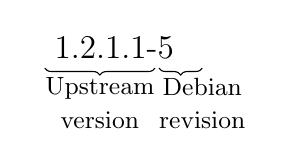
\begin{tikzpicture}
  \draw (0,0) node[above right] {\large 1.2.1.1-5};
  \draw [decorate,decoration={brace}] (2,0) -- (1.45,0) node[at start,below,text width=1.6cm,text centered] {\small  Debian revision};
  \draw [decorate,decoration={brace}] (1.4,0) -- (0,0) node[midway,below,text width=1.6cm,text centered] { \small Upstream version};
\end{tikzpicture}
\end{center}
\begin{itemize}
\item $B<j$G=$@5$9$k$+(B \texttt{dch} $B%3%^%s%I$r;HMQ$9$k(B
\item Debian $B$b$7$/$O(B Ubuntu $B$N(B Bug $B$r(B close $B$9$kFCJL$J=q<0(B\newline
  Debian: \texttt{Closes:~\#595268}; Ubuntu: \texttt{LP:~\#616929}
\end{itemize}
  \seprule
  \begin{lstlisting}[basicstyle=\ttfamily\footnotesize]
mpich2 (1.2.1.1-5) unstable; urgency=low

  * Use /usr/bin/python instead of /usr/bin/python2.5. Allow
    to drop dependency on python2.5.  Closes: #595268
  * Make /usr/bin/mpdroot setuid. This is the default after
    the installation of mpich2 from source, too. LP: #616929
    + Add corresponding lintian override.

 -- Lucas Nussbaum <lucas@debian.org>  Wed, 15 Sep 2010 18:13:44 +0200
\end{lstlisting}
\paragraph{\ttfamily{debian/control}}
\label{sec-2-7}

\begin{itemize}
\item $B%Q%C%1!<%8$N%a%?%G!<%?(B
\begin{itemize}
\item $B%=!<%9%Q%C%1!<%8K\BN(B
\item $B:n@.$9$k%P%$%J%j%Q%C%1!<%8A4$F(B
\end{itemize}
\item Package name, section, priority, maintainer, uploaders,
  build-dependencies, dependencies, description, homepage, \ldots{}
\item Debian $B%]%j%7!<(B $BBh(B 5 $B>O;2>H(B:\newline
  \href{http://www.debian.org/doc/debian-policy/ch-controlfields.html}{http://www.debian.org/doc/debian-policy/ch-controlfields.html}
\end{itemize}
  \seprule
\begin{lstlisting}[basicstyle=\ttfamily\footnotesize]
Source: wget
Section: web
Priority: important
Maintainer: Noel Kothe <noel@debian.org>
Build-Depends: debhelper (>> 5.0.0), gettext, texinfo,
 libssl-dev (>= 0.9.8), dpatch, info2man
Standards-Version: 3.8.4
Homepage: http://www.gnu.org/software/wget/

Package: wget
Architecture: any
Depends: ${shlibs:Depends}, ${misc:Depends}
Description: retrieves files from the web
 Wget is a network utility to retrieve files from the Web
\end{lstlisting}
\paragraph{Architecture: all or any}
\label{sec-2-8}

$BFs<oN`$N%P%$%J%j%Q%C%1!<%8(B
\begin{itemize}
\item $B%"!<%-%F%/%A%cKh$KFbMF$,0[$J$k%Q%C%1!<%8(B
\begin{itemize}
\item $BNc(B: C $B%W%m%0%i%`(B
\item \texttt{debian/control} $B$G$O(B \texttt{Architecture: any}
\begin{itemize}
\item $B$b$7$/$O(B, $B%"!<%-%F%/%A%c$N%5%V%;%C%HKh$K;XDj(B:\newline
      \texttt{Architecture:\ amd64 i386 ia64 hurd-i386}
\end{itemize}
\item \texttt{buildd.debian.org}$B$G%"%C%W%m!<%I$7$?%"!<%-%F%/%A%c0J30$K$D$$$F%Q%C%1!<%8$r:n@.(B
\item $B%Q%C%1!<%8L>(B: \texttt{\textsl{package}\_\textsl{version}\_\textsl{architecture}.deb}
\end{itemize}
\item $B%"!<%-%F%/%A%c$K$h$i$:Cf?H$,F1$8%Q%C%1!<%8(B
\begin{itemize}
\item $BNc(B: Perl $B%i%$%V%i%j(B
\item \texttt{debian/control} $B$G$O(B \texttt{Architecture: all}
\item $B%Q%C%1!<%8L>(B: \texttt{\textsl{package}\_\textsl{version}\_\textbf{all}.deb}
\end{itemize}
\end{itemize}
$B0l$D$N%=!<%9%Q%C%1!<%8$+$i(B, $BJ#?t$N(B
  \texttt{Architecture:\ any} $B$H(B
  \texttt{Architecture:\ all} $B$N%P%$%J%j%Q%C%1!<%8$r@8@.$9$k$3$H$,2DG=(B
\paragraph{\ttfamily{debian/rules}}
\label{sec-2-9}

\begin{itemize}
\item Makefile
\item Debian$B%Q%C%1!<%8$r:n@.$9$k(B interface
\item Debian $B%]%j%7!<$N(B $BBh(B4$B>O(B 8 $B@a(B $B;2>H(B
  {\small \texttt{http://www.debian.org/doc/debian-policy/ch-source.html\#s-debianrules}}
\item 5 $B$D$NI,?\%?!<%2%C%H(B:
\begin{itemize}
\item \texttt{build}: $B%Q%C%1!<%8$N@_Dj$H9=C[$r<B9T(B
\item \texttt{binary, binary-arch, binary-indep}: $B%P%$%J%j%Q%C%1!<%8$N:n@.(B
\begin{itemize}
\item \texttt{dpkg-buildpackage} $B$O(B
      \texttt{binary} $B$rA4$F$N%Q%C%1!<%8$K$D$$$F(B,
      \texttt{binary-arch} $B$r(B \texttt{Architecture: any} $B$N%Q%C%1!<%8$K$D$$$F(B
      $B$=$l$>$l<B9T(B
\end{itemize}
\item \texttt{clean}: $B%=!<%9%G%#%l%/%H%j$N(B clean up
\end{itemize}
\end{itemize}
\paragraph{$B%Q%C%1!<%8:n@.;Y1g(B}
\label{sec-2-10}

\begin{itemize}
\item \texttt{debian/rules} $B$K(B shell $B%9%/%j%W%H$rD>@\5-=R2DG=(B
\begin{itemize}
\item $BNc(B: \texttt{adduser} $B%Q%C%1!<%8(B
\end{itemize}
\item $BNI$$J}K!(B: \textsl{Packaging helper} $B$N;HMQ(B
\item $BNI$/;H$o$l$k$N$O(B \textbf{debhelper} ($B%Q%C%1!<%8$N(B 98\% $B$G;HMQCf(B)
\item $BL\E*(B:
\begin{itemize}
\item $BA4$F$N%Q%C%1!<%8$G;HMQ$5$l$kI8=`E*$J%D!<%k$N8F=P$7$r6&DL2=(B
\item $B%Q%C%1!<%8:n@.;~$N%P%0$r$7$C$+$j$H=$@5(B\newline
    {\footnotesize
    dh\_installdirs, dh\_installchangelogs, dh\_installdocs,
    dh\_installexamples, dh\_install, dh\_installdebconf, dh\_installinit,
    dh\_link, dh\_strip, dh\_compress, dh\_fixperms, dh\_perl,
    dh\_makeshlibs, dh\_installdeb, dh\_shlibdeps, dh\_gencontrol,
    dh\_md5sums, dh\_builddeb,} ...
\item \texttt{debian/rules} $B$G$3$l$i$r8F$V(B
\item \texttt{debian/} $B0J2<$K%U%!%$%k$rCV$$$F@_Dj$9$k(B\newline
    {\footnotesize
    \ttfamily dirs, \textsl{package}.docs, \textsl{package}.examples,
    \textsl{package}.install, \textsl{package}.manpages }...
\item Third-party $B%X%k%Q!<$b$"$k(B: \textalert{python-support}, \textalert{dh\_ocaml} \ldots{}
\item \texttt{debian/compat}: debhelper $B$NE,MQ$9$k%P!<%8%g%s(B(``7'' $B$r;H$*$&(B)
\end{itemize}
\end{itemize}
\paragraph{\ttfamily{debian/rules} using debhelper(1/2)}
\label{sec-2-11}

  \begin{lstlisting}[basicstyle=\ttfamily\footnotesize]
#!/usr/bin/make -f

# Uncomment this to turn on verbose mode.
#export DH_VERBOSE=1

build:
        $(MAKE)
        #docbook-to-man debian/packagename.sgml > packagename.1

clean:
        dh_testdir
        dh_testroot
        rm -f build-stamp configure-stamp
        $(MAKE) clean
        dh_clean

install: build
        dh_testdir
        dh_testroot
        dh_clean -k
        dh_installdirs
        # Add here commands to install the package into debian/packagename.
        $(MAKE) DESTDIR=$(CURDIR)/debian/packagename install
\end{lstlisting}
\paragraph{\ttfamily{debian/rules} using debhelper(2/2)}
\label{sec-2-12}

  \begin{lstlisting}[basicstyle=\ttfamily\footnotesize]

# Build architecture-independent files here.
binary-indep: build install

# Build architecture-dependent files here.
binary-arch: build install
        dh_testdir
        dh_testroot
        dh_installchangelogs
        dh_installdocs
        dh_installexamples
        dh_install
        dh_installman
        dh_link
        dh_strip
        dh_compress
        dh_fixperms
        dh_installdeb
        dh_shlibdeps
        dh_gencontrol
        dh_md5sums
        dh_builddeb

binary: binary-indep binary-arch
.PHONY: build clean binary-indep binary-arch binary install configure
\end{lstlisting}
\paragraph{CDBS}
\label{sec-2-13}

\begin{itemize}
\item \texttt{debhelper} $B$rMQ$$$F$b$=$l$J$j$K>iD9(B
\item $B6&DL$N5!G=$KJ,$1$?FsCJL\$N(B helper $B$,$"$k(B
\begin{itemize}
\item \texttt{./configure \&\& make \&\& make install} $B$d(B CMake
\item Perl, Python, Ruby, GNOME, KDE, Java, Haskel, \ldots{}
\end{itemize}
\item CDBS
\begin{itemize}
\item 2005 $BG/$KF3F~(B. \textsl{GNU make} $B$K$h$k=hJ}d5(B
\item $B%I%-%e%a%s%H(B: \texttt{/usr/share/doc/cdbs/}
\item $B$7$+$7$J$,$i(B, $B$3$l$r7y$&3+H/<T$b$$$k(B
\begin{itemize}
\item $B%Q%C%1!<%8$r%+%9%?%^%$%:$7$F9=C[$9$k$N$,:$Fq(B:\\
``\textsl{twisty maze of makefiles and environment variables}''
\item $BAG$N(B debhelper $B$KHf$Y$FCY$$(B($BITMW$J(B \texttt{dh\_*} $B$N8F$S=P$7$,B?$$(B)
\end{itemize}
\end{itemize}
\end{itemize}
  \seprule
      \begin{lstlisting}[basicstyle=\ttfamily\footnotesize]
#!/usr/bin/make -f
include /usr/share/cdbs/1/rules/debhelper.mk
include /usr/share/cdbs/1/class/autotools.mk

# add an action after the build
build/mypackage::
    /bin/bash debian/scripts/foo.sh
      \end{lstlisting}
\paragraph{Dh (a.k.a Debhelper 7, or dh7)}
\label{sec-2-14}

\begin{itemize}
\item 2008 $BG/$K(B \textsl{CDBS killer} $B$H$7$FF3F~(B
\item \textalert{dh} $B%3%^%s%I$O(B \texttt{dh\_*} $B$r8F$S=P$9(B
\item \textsl{debian/rules} $B$KI,MW$J$N$O(B overrides $B$N$_(B
\item CDBS $B$KHf$Y$F%+%9%?%^%$%:$,MF0W(B
\item $B%I%-%e%a%s%H(B:man (\texttt{debhelper(7)}, \texttt{dh(1)}), DebConf9 $B$G$NH/I=%9%i%$%I(B\\
\href{http://kitenet.net/~joey/talks/debhelper/debhelper-slides.pdf}{http://kitenet.net/\~joey/talks/debhelper/debhelper-slides.pdf}
\end{itemize}
  \seprule
    \begin{lstlisting}[basicstyle=\ttfamily\footnotesize]
#!/usr/bin/make -f
%:
    dh $@

override_dh_auto_configure:
     dh_auto_configure -- --with-kitchen-sink

override_dh_auto_build:
     make world

    \end{lstlisting}%$
\paragraph{classic debhelper v.s. CDBS v.s. dh}
\label{sec-2-15}

\begin{itemize}
\item $B8=>u$N;HMQN((B:
\begin{itemize}
\item classic debhelper: 41\% \hskip 1em CDBS: 23\% \hskip 1em  dh: 34\%
\end{itemize}
\item $B$I$l$r3X$V$Y$-$+(B?
\begin{itemize}
\item $BB?J,A4It$r$=$l$J$j$K(B
\item dh $B$b$7$/$O(B CDBS $B$r;H$&>l9g$K$O(B debhelper $B$NCN<1$,I,MW(B
\item CDBS $B$r;H$C$F$$$k%Q%C%1!<%8$r=$@5$9$kI,MW$,$"$k(B
\end{itemize}
\item $B?7$7$$%Q%C%1!<%8$K$O$I$l$r;H$&$Y$-$+(B?
\begin{itemize}
\item \textalert{dh} ($BB?J,$3$l$+$iA}$($F$$$/(B)
\end{itemize}
\end{itemize}
\begin{center}
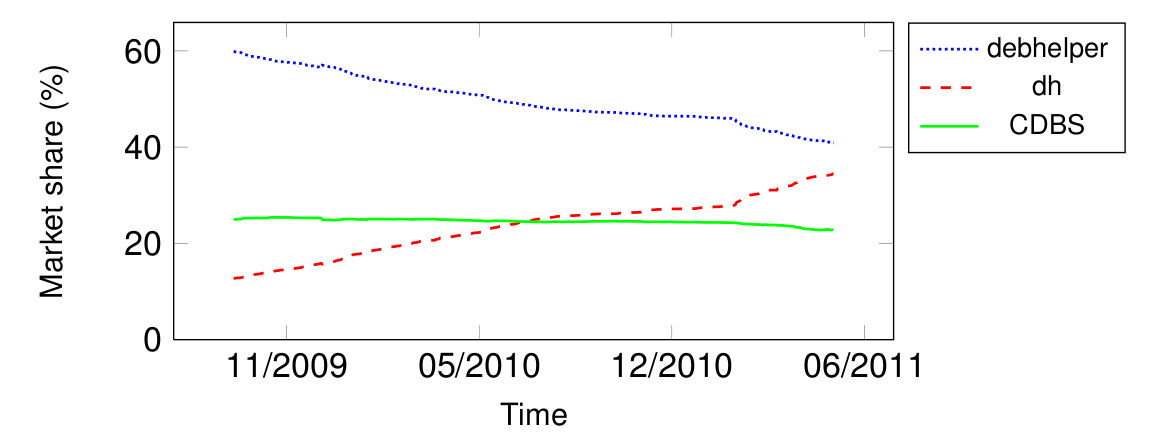
\includegraphics[width=9cm]{image201108/debhelper-cdbs-dh.png}
\end{center}

%  \begin{center}
%    \begin{tikzpicture}
%\begin{axis}[small,label style={font=\footnotesize},xlabel={\small Time},ylabel={\small $B;HMQN((B (\%)},
%   date coordinates in=x,height=4.85cm,width=9cm,xticklabel={\month/\year},
%        legend style={font=\footnotesize,at={(1.02,1)},anchor=north west},max space between ticks=82,try min ticks=5,ymin=0]
%   \addplot[mark=none,blue,thick,style=densely dotted] table[x=date,y=dh] {cdbs-dh7.txt};
%   \addplot[mark=none,red,thick,style=dashed] table[x=date,y=dh7] {cdbs-dh7.txt};
%   \addplot[mark=none,green,thick] table[x=date,y=cdbs] {cdbs-dh7.txt};
%   \legend{debhelper, dh, CDBS}
%\end{axis}
%\end{tikzpicture}
%\end{center}
\subsection*{$B%Q%C%1!<%8$N9=C[(B, $B%F%9%H(B}
\label{sec-3}
\paragraph{$B%Q%C%1!<%8$N9=C[(B}
\label{sec-3-1}

\begin{itemize}
\item \texttt{apt-get build-dep mypackage}\newline
  \texttt{Build-Depends} $B$K$"$k%Q%C%1!<%8$r%$%s%9%H!<%k$9$k(B
\item \texttt{debuild}: $B%Q%C%1!<%8$N9=C[(B, \texttt{lintian} $B$K$h$k%A%'%C%/(B, GPG $B%5%$%s(B
\begin{itemize}
\item $B$b$7$/$O(B \texttt{dpkg-buildpackage -us -uc} $B$rD>@\<B9T(B
\end{itemize}
\item $B%Q%C%1!<%8$O%/%j!<%s$+$D:G>.9=@.$N4D6-$G%F%9%H$9$k$N$,NI$$(B
\begin{itemize}
\item \texttt{pbuilder}: \textsl{chroot} $B4D6-2<$G%Q%C%1!<%8$r%S%k%I$9$k%X%k%Q!<(B\newline
    $BNI$$%I%-%e%a%s%H(B: \href{https://wiki.ubuntu.com/PbuilderHowto}{https://wiki.ubuntu.com/PbuilderHowto} \newline
    (\textttc{cowbuilder}, \textttc{ccache}, \textttc{distcc} $B$K$h$k:GE,2=$J$I(B)
\item \texttt{schroot} $B$H(B \texttt{sbuild}: Debian $B$N(B build daemon $B$G;HMQ(B\newline
    (\texttt{pbuilder}$B$[$I%7%s%W%k$G$O$J$$$1$l$I(B LVM snapshot $B$,;H$($?$j$9$k(B\newline
    $B%I%-%e%a%s%H(B: \href{https://help.ubuntu.com/community/SbuildLVMHowto}{https://help.ubuntu.com/community/SbuildLVMHowto})
\end{itemize}
\item \texttt{.deb} $B%U%!%$%k$H(B \texttt{.changes} $B%U%!%$%k$r@8@.$9$k(B
\begin{itemize}
\item \texttt{.changes}: $B2?$r@8@.$7$?$N$+$,5-=R$5$l$k(B. upload $B;~$K;HMQ$9$k(B
\end{itemize}
\end{itemize}
\paragraph{$B%Q%C%1!<%8$N%$%s%9%H!<%k(B, $B%F%9%H(B}
\label{sec-3-2}

\begin{itemize}
\item $B%m!<%+%k$K%$%s%9%H!<%k$9$k(B: \textttc{debi}\newline
  \texttt{.changes} $B%U%!%$%k$r;HMQ$7$F2?$r%$%s%9%H!<%k$7$?$+3NG'(B
\item $B%Q%C%1!<%8$NCf?H$N3NG'(B: \texttt{debc ../mypacakge<TAB>.changes}
\item $B0JA0$N%P!<%8%g%s$H$NHf3S(B: \newline
  \texttt{debdiff ../mypackage\_1\_*.changes ../mypackage\_2\_*.changes} \newline
  $B%=!<%9%Q%C%1!<%8$NHf3S$O(B \newline
  \texttt{debdiff ../mypackage\_1\_*.dsc ../mypackage\_2\_*.dsc}
\item \texttt{lintian} $B$K$h$k%A%'%C%/(B:
  \texttt{lintian -i ../mypackage<TAB>.changes}\newline
  \texttt{lintian -i}: $B%(%i!<$K$D$$$F>\:Y$K>pJs$rDs6!(B
\item Debian $B$X%Q%C%1!<%8$r%"%C%W%m!<%I(B: \textttc{dput}
\item $B8D?ME*$J%Q%C%1!<%8%j%]%8%H%j$N:n@.(B: \textttc{reprepro}\newline
  $B%I%-%e%a%s%H(B: \href{http://mirror.alioth.debian.org}{http://mirror.alioth.debian.org}
\end{itemize}
\subsection*{$B<B=,(B1: grep $B%Q%C%1!<%8$N=$@5(B}
\label{sec-4}
\paragraph{$B<B=,(B1: grep $B%Q%C%1!<%8$N=$@5(B}
\label{sec-4-1}

\begin{itemize}
\item \href{http://ftp.jp.debian.org/debian/pool/main/g/grep/}{http://ftp.jp.debian.org/debian/pool/main/g/grep/} $B$+$i(B 2.6.3-3 $B$r<hF@(B
\item $BE83+$7$F(B \texttt{debian/} $B0J2<$r8+$F$_$h$&(B
\begin{itemize}
\item $B4v$D$N%P%$%J%j%Q%C%1!<%8$,@8@.$5$l$F$$$^$9$+(B?
\item $B$I$N%Q%C%1!<%8%X%k%Q!<$,;HMQ$5$l$F$$$^$9$+(B?
\end{itemize}
\item $B%Q%C%1!<%8$N:n@.(B
\item $B%Q%C%1!<%8$N=$@5(B: chengelog $B$N%(%s%H%j$r0l8DA}$d$7$F$_$h$&(B!
\item \texttt{./configure} $B$G(B perl-regexp support $B$rL58z2=$7$F$_$h$&(B
\item $B%Q%C%1!<%8$N:F9=C[(B
\item debdiff $B$G%*%j%8%J%k$H?7$7$$%Q%C%1!<%8$NHf3S$7$F$_$h$&(B
\item $B?7$7$/:n@.$7$?%Q%C%1!<%8$r%$%s%9%H!<%k$7$F$_$h$&(B
\end{itemize}

$B5?Ld(B/$B<ALd$J$I$"$C$?$iD>$0$K8@$C$F2<$5$$(B.
\subsection*{$B0lJb?J$s$@OCBj(B}
\label{sec-5}
\paragraph{\ttfamily{debian/copyright}}
\label{sec-5-1}

\begin{itemize}
\item $B%=!<%9$H%Q%C%1!<%8$K4X$9$k(B Copyright $B$H%i%$%;%s%9$N>pJs(B
\item $BEAE}E*$K$OC1$J$k(B text $B$G5-=R(B
\item $B?7(B: machine-readble format $B$N:vDj(B: \href{http://dep.debian.net/deps/dep5/}{http://dep.debian.net/deps/dep5/}
\end{itemize}
  \seprule
  \begin{lstlisting}[basicstyle=\ttfamily\footnotesize]
Format: <VERSIONED_FORMAT_URL>
Upstream-Name: X Solitaire
Source: ftp://ftp.example.com/pub/games

Files: *
Copyright: Copyright 1998 John Doe <jdoe@example.com>
License: GPL-2+
 This program is free software; you can redistribute it
 [...]
 .
 On Debian systems, the full text of the GNU General Public
 License version 2 can be found in the file
 `/usr/share/common-licenses/GPL-2'.

Files: debian/*
Copyright: Copyright 1998 Jane Smith <jsmith@example.net>
License:
 [LICENSE TEXT]
\end{lstlisting}
\paragraph{$B>eN.$N%=!<%9$N=$@5(B}
\label{sec-5-2}

\begin{itemize}
\item $BIQHK$K9T$J$o$l$F$$$k(B
\begin{itemize}
\item $B%P%0=$@5(B, Debian $B8GM-$N%+%9%?%^%$%:(B
\item $B?7$7$$(B upstream release $B$+$i$N(B backport
\end{itemize}
\item $B4v$D$+$NJ}K!$,$"$k(B
\begin{itemize}
\item $B%U%!%$%k$rD>@\=$@5$9$k(B
\begin{itemize}
\item $B$3$l$O(B simple
\item $B$7$+$7$J$,$i(B, $BJQ99E@$NDI@W$dJ8=q2=$,$G$-$J$$(B
\end{itemize}
\item patch $B%7%9%F%`(B
\begin{itemize}
\item upstream $B$X$N9W8%(B
\item $BGI@8%G%#%9%H%j%S%e!<%7%g%s$H$NJQ99E@$N6&M-(B
\item $BJQ99E@$rL@$i$+$K(B\newline
      \href{http://patch-tracker.debian.org/}{http://patch-tracker.debian.org/}
\end{itemize}
\end{itemize}
\end{itemize}
\paragraph{Patch $B%7%9%F%`(B}
\label{sec-5-3}

\begin{itemize}
\item $B86B'(B: $BJQ99E@$O%Q%C%A$H$7$F(B \texttt{debian/patches/} $B$KCV$/(B
\item $B9=C[;~$KE,MQ$7$?$j30$7$?$j$9$k(B
\item $B$3$l$^$G$O(B: $B4v$D$+$N<BAu(B\newline
  \textsl{simple-patchsys}(\textsl{cdbs}),
  \textsl{dpatch}, \textttc{\textsl{quilt}}
\item $B$3$l$i$OA4$FFs$D$N(B \texttt{debian/rules} $B$N%?!<%2%C%H$r%5%]!<%H(B:
\begin{itemize}
\item \texttt{debian/rules patch}: $BA4$F$N%Q%C%A$rE,MQ(B
\item \texttt{debian/rules unpatch}: $BA4$F$N%Q%C%A$r30$9(B
\end{itemize}
\item $B$5$i$J$k%I%-%e%a%s%H(B: \href{http://wiki.debian.org/debian/patches}{http://wiki.debian.org/debian/patches}
\item \textalert{$B%Q%C%A%7%9%F%`F~$j$N?7$7$$%=!<%9%U%)!<%^%C%H(B: 3.0 (quilt)}
\begin{itemize}
\item $B$3$l$+$i$N?d>)$5$l$kJ}K!(B
\item \textsl{quilt} $B$K$D$$$FCN$kI,MW$,$"$k(B\newline
    \href{http://pkg-perl.alioth.debian.org/howtow/quilt.html}{http://pkg-perl.alioth.debian.org/howtow/quilt.html}
\end{itemize}
\end{itemize}
\paragraph{Patch $B$K4X$9$k%I%-%e%a%s%H(B}
\label{sec-5-4}

\begin{itemize}
\item $B%Q%C%A$N@hF,$KI8=`E*$J%X%C%@$H$7$F5-=R(B
\item Patch Tagging Guideline: \href{http://deb.debian.net/deps/dep3/}{http://deb.debian.net/deps/dep3/}
\item $BA4$F$N%Q%C%A$O(B \href{http://patch-tracker.debian.org}{http://patch-tracker.debian.org} $B$K$F8x3+$5$l$F$$$k(B
\end{itemize}
\seprule
  \begin{lstlisting}[basicstyle=\ttfamily\footnotesize]
Description: Fix widget frobnication speeds
        Frobnicating widgets too quickly tended to cause explosions.
Forwarded: http://lists.example.com/2010/03/1234.html
Author: John Doe <johndoe-guest@users.alioth.debian.org>
Applied-Upstream: 1.2, http://bzr.foo.com/frobnicator/revision/123
Last-Update: 2010-03-29

--- a/src/widgets.c
+++ b/src/widgets.c
@@ -101,9 +101,6 @@ struct {
\end{lstlisting}
\paragraph{$B%$%s%9%H!<%k(B/$B%j%`!<%V;~$K2?$+$r9T$J$&$K$O(B?}
\label{sec-5-5}

\begin{itemize}
\item $B%Q%C%1!<%8$rE83+$9$k$@$1$G$OIT==J,$J;~$,$"$k(B
\item $B%7%9%F%`%f!<%6$r:n@.(B/$B:o=|$7$?$j(B, $B%5!<%S%9$r3+;O(B/$BDd;_$5$;$?$j(B, \textsl{alternatives} $B$r4IM}$7$?$j(B
\item $B$3$l$i$O(B \textsl{$B%a%s%F%J%9%/%j%W%H(B} $B$G9T$J$&(B\newline
  \texttt{preinst, postinst, prerm, postrm}
\begin{itemize}
\item $B6&DL$NF0:n$K4X$9$k(B snippet $B$O(B debhelper $B$G@8@.$5$l$k(B
\end{itemize}
\item $B%I%-%e%a%s%H(B: Debian Policy, $BBh(B6$B>O(B\\
{\footnotesize \url{http://www.debian.org/doc/debian-policy/ch-maintainerscripts.html}} \newline
\item $B%I%-%e%a%s%H(B: Debian Developer's Reference, $BBh(B6$B>O(B 4 $B@a(B\\
{\scriptsize \url{http://www.debian.org/doc/developers-reference/best-pkging-practices.html}} \newline
  {\footnotesize \url{http://people.debian.org/~srivasta/MaintainerScripts.html}}
\item $B%f!<%6$X$N%W%m%s%W%H$NI=<((B
\begin{itemize}
\item \textalert{debconf} $B$G9T$J$&(B
\item $B%I%-%e%a%s%H(B: \texttt{debconf-devel(7)} (\texttt{debconf-doc} package)
\end{itemize}
\end{itemize}
\paragraph{upstream $B$N%P!<%8%g%s4F;k(B}
\label{sec-5-6}

\begin{itemize}
\item \texttt{debian/watch} $B$K5-=R$7$F$*$/(B (\texttt{uscan(1)} $B$r;2>H(B)
\end{itemize}
    \begin{lstlisting}[basicstyle=\ttfamily\footnotesize]
version=3
http://tmrc.mit.edu/mirror/twisted/Twisted/(\d\.\d)/ \
  Twisted-([\d\.]*)\.tar\.bz2
    \end{lstlisting}
\begin{itemize}
\item \texttt{debian/watch} $B$r;HMQ$7$F4F;k$9$k(B Debian $B$N%$%s%U%i(B:\newline
  \href{http://dehs.alioth.debian.org}{http://dehs.alioth.debian.org}
\item Package Tracking System $B$+$i$N%a%s%F%J$X%a!<%k$K$h$kDLCN(B:\newline
  \href{http://packages.qa.debian.org/}{http://packages.qa.debian.org/}
\item \texttt{uscan}: $B<jF0%A%'%C%/(B
\item \texttt{uupdate}: $B:G?7$N(B upstream $B%=!<%9$rMQ$$$F<+F0%"%C%W%G!<%H$r;n$_$k(B
\end{itemize}
\paragraph{VCS(e.g. SVN, Git) $B$rMQ$$$?%Q%C%1!<%8%s%0(B}
\label{sec-5-7}

\begin{itemize}
\item $B%V%i%s%A$d%?%0IU$1$J$I(B, $B%Q%C%1!<%8:n@.:n6H$r=u$1$k4v$D$+$N%D!<%k(B:\newline
    \texttt{svn-buildpackage}, \texttt{git-buildpackage}
\item $BNc(B: \texttt{git-buildpackage}
\begin{itemize}
\item \texttt{upstream} branch to track upstream with \texttt{upstream/\textsl{version}} tags
\item \texttt{master} branch tracks the Debian package
\item \texttt{debian/\textsl{version}} tags for each upload
\item \texttt{pristine-tar} branch to be able to rebuild the upstream tarball
\end{itemize}
\item \texttt{debian/control} $BFb$N(B \texttt{Vcs-*} fields $B$G%j%]%8%H%j$N>l=j$r5-=R(B
\begin{itemize}
\item \href{http://wiki.debian.org/Alioth/Git}{http://wiki.debian.org/Alioth/Git}
\item \href{http://wiki.debian.org/Alioth/Svn}{http://wiki.debian.org/Alioth/Svn}
\end{itemize}
\end{itemize}
  \begin{lstlisting}[basicstyle=\ttfamily\footnotesize]
Vcs-Browser: http://git.debian.org/?p=devscripts/devscripts.git
Vcs-Git: git://git.debian.org/devscripts/devscripts.git
  \end{lstlisting}
  \begin{lstlisting}[basicstyle=\ttfamily\footnotesize]
Vcs-Browser: http://svn.debian.org/viewsvn/pkg-perl/trunk/libwww-perl/
Vcs-Svn: svn://svn.debian.org/pkg-perl/trunk/libwww-perl
  \end{lstlisting}
\begin{itemize}
\item VCS $B$H$N$d$j$H$j(B: \texttt{debcheckout}, \texttt{debcommit}
\begin{itemize}
\item \texttt{debcheckout grep} $\rightarrow$ checks out the source package from Git
\end{itemize}
\end{itemize}
\subsection*{Debian $B%Q%C%1!<%8$N%a%s%F%J%s%9(B}
\label{sec-6}
\paragraph{Debian $B$K9W8%$9$k4v$D$+$NJ}K!(B}
\label{sec-6-1}

\begin{itemize}
\item $B$b$C$H$bNI$/$J$$J}K!(B:
\begin{itemize}
\item $BFH<+%=%U%H%&%'%"$r%Q%C%1!<%8%s%0(B
\item $B$=$l$r(BDebian$B$KF~$l$k(B
\item $B%H%s%:%i$3$/(B
\end{itemize}
\item $B8=:_%a%s%F$5$l$F$$$J$$%Q%C%1!<%8(B((\textsl{orphaned packages})$B$r$R$-$H$k(B
\begin{itemize}
\item Debian $B$K$O%a%s%F$5$l$F$$$J$$B?$/$N%Q%C%1!<%8$,$"$k(B
\item $B$"$J$?$,IaCJ;HMQ$7$F$$$k%Q%C%1!<%8$,$=$&$+$b$7$l$J$$(B!
\end{itemize}
\item $B%Q%C%1!<%8%s%0%A!<%`$K;22C$7$h$&(B
\begin{itemize}
\item $B%Q%C%1!<%8%s%0$K%U%)!<%+%9$7$?4v$D$b$N%A!<%`$,$"$k(B. $B=u$1$rI,MW$H$7$F$$$k(B
\item $B8=:_$N%A!<%`$N0lMw(B: \href{http://wiki.debian.org/Teams}{http://wiki.debian.org/Teams}
\item $B$h$j7P83K-IY$J9W8%<T$+$i3X$VAG@2$i$7$$J}K!(B!
\end{itemize}
\item $B?7$7$$%=%U%H%&%'%"$r(B Debian $B$KF~$l$k$J$i(B
\begin{itemize}
\item $B$G$-$l$P==J,M-MQ$G6=L#?<$$%=%U%H%&%'%"$@$1$K$7$F$[$7$$(B
\item $BBeMQIJ$,4{$K(B Debian $B$K$"$C$?$j$7$J$$$+$$(B?
\end{itemize}
\end{itemize}
\paragraph{Ubuntu $B$K6=L#$,$*$"$j$G$9$+(B?}
\label{sec-6-2}

\begin{itemize}
\item Ubuntu $B$O(B Debian $B$NGI@8J*$r<g$K4IM}$7$F$$$^$9(B
\item $BFCDj$N%Q%C%1!<%8$KCmL\$;$:(B, Debian $B$N%A!<%`$H6&F1:n6H$r$7$F$$$^$9(B.
\item $BBgDq$N>l9g(B, $B?7$7$$%Q%C%1!<%8$O@h$:(B Debian $B$K%"%C%W%m!<%I$9$k$3$H$r?d>)(B:\newline
  \href{https://wiki.ubuntu.com/UbuntuDevelopment/NewPackages}{https://wiki.ubuntu.com/UbuntuDevelopment/NewPackages}
\item $BB?J,NI$$J}K!$O(B\ldots{}
\begin{itemize}
\item Debian $B$N%A!<%`$K;22C$7$F(B Ubuntu $B$H$N66EO$7$r$9$k(B
\item $BJ,4t$r8:$i$9:n6H(B. Launchpad $B$N%P%0$N%H%j%"!<%8(B
\item $BB?$/$N(B Debian $B$N%D!<%k$,Lr$KN)$D$G$7$g$&(B:
\begin{itemize}
\item Ubuntu column on the Developer's packages overview
\item Ubuntu box on the Package Tracking System
\item Receive launchpad bugmail via the PTS
\end{itemize}
\end{itemize}
\end{itemize}
\paragraph{$B$_$J$7$4%Q%C%1!<%8$N0z$-<h$j(B}
\label{sec-6-3}

\begin{itemize}
\item $BA4$F$N%j%9%H(B: \href{http://www.debian.org/devel/wnpp/}{http://www.debian.org/devel/wnpp/}
\item \texttt{wnpp-alert} $B$r%$%s%9%H!<%k$7$h$&(B
\item $B0[$J$k%9%F!<%?%9(B
\begin{itemize}
\item \textalert{O}rphaned: \newline
    $B%Q%C%1!<%8$O%a%s%F$5$l$F$$$J$$(B. $B<+M3$K0z$-<h$l$k(B
\item \textalert{RFA}: \textalert{R}equest \textalert{F}or \textalert{A}dopter \newline
    $B%a%s%F%J$ON$?F$rC5$7$F$$$k$,(B, $B8=;~E@$G$O%a%s%F$O7QB3$7$F9T$J$C$F$$$k(B.
    $B0z$-<h$j$O<+M3(B. $B8=%a%s%F%J$X%a!<%k$9$k$N$,NI$$(B.
\item \textalert{ITA}: \textalert{I}ntent \textalert{T}o \textalert{A}dopt \newline
    $BC/$+$,%Q%C%1!<%8$r0z$-<h$j$r@k8@$7$?>uBV(B. $B<j=u$1$r?=$7=P$k$3$H$O$G$-$k(B.
\item \textalert{RFH}: \textalert{R}equest \textalert{F}or \textalert{H}elp \newline
    $B%a%s%F%J$,=u$1$r5a$a$F$$$k>uBV(B
\end{itemize}
\item $B5?LdE@$,$"$l$P(B \texttt{debian-qa@lists.debian.org}, $B$b$7$/$O(B
  \texttt{irc.debian.org} $B$N(B \texttt{\#debian-qa} $B$GLd$$9g$o$;$r(B!
\end{itemize}
\paragraph{$B:n@.$7$?%Q%C%1!<%8$r(B Debian $B$KF~$l$k$K$O(B?}
\label{sec-6-4}

\begin{itemize}
\item $B%Q%C%1!<%8$r(B Debian $B$KF~$l$k$N$K$O8x<0$J%9%F!<%?%9$OITMW$G$9(B
\begin{enumerate}
\item $B%=!<%9%Q%C%1!<%8$N=`Hw$r$9$k(B
\item $B%Q%C%1!<%8$N%9%]%s%5!<$K$J$C$F$/$l$k(B Debian Developer $B$rC5$9(B
\end{enumerate}
\item $B8x<0$J%9%F!<%?%9(B:
\begin{itemize}
\item \textbf{Debian Maintainer(DM)}: \newline
    $B<+J,$N%Q%C%1!<%8$r%"%C%W%m!<%I$9$k8"8B$r;}$D3+H/<T(B\newline
    \href{http://wiki.debian.org/DebianMaintainer}{http://wiki.debian.org/DebianMaintainer} $B;2>H(B
\item \textbf{Debian Developer(DD)}: \newline
    Debian $B%W%m%8%'%/%H$N%a%s%P!<(B.
   $BEjI<8"$r;}$A(B, $B$I$s$J%Q%C%1!<%8$G$b%"%C%W%m!<%I2DG=(B
\end{itemize}
\end{itemize}
\paragraph{$B=u$1$rF@$k$K$O(B?}
\label{sec-6-5}

\begin{itemize}
\item Help you will need:
\begin{itemize}
\item $B$"$J$?$N<ALd$KBP$7$FEz$H=u8@$r$/$l$F(B, $B%3!<%I$b%l%S%e!<$7$F$/$l$F(B
\item $B%Q%C%1!<%8$N=`Hw$,$G$-$?$i%9%]%s%5!<$K$b$J$C$F$/$l$F(B
\end{itemize}
\item You can get help from:
\begin{itemize}
\item $B%Q%C%1!<%8%s%0%A!<%`$NB>$N%a%s%P!<(B: $B:G$bNI$$J}K!(B
\begin{itemize}
\item $B$"$J$?$N%Q%C%1!<%88GM-$N;vJA$K$D$$$FCN$C$F$$$k(B
\item $B%A!<%`$N%a%s%P!<$K$"$J$?$O$J$l$k(B
\item \href{http://wiki.debian.org/Teams}{http://wiki.debian.org/Teams} $B;2>H(B
\end{itemize}
\item Debian Mentors $B%0%k!<%W(B($B$b$7%Q%C%1!<%8$,9g$&%A!<%`$,L5$$$J$i(B)
\begin{itemize}
\item \href{http://wiki.debian.org/DebianMentorsFaq}{http://wiki.debian.org/DebianMentorsFaq}
\item ML: \hyperref[debian-mentors-lists.debian.org]{debian-mentors@lists.debian.org}
\item IRC: \texttt{\#debian-mentors} on \texttt{irc.debian.org}
\item \href{http://mentors.debian.net}{http://mentors.debian.net}
\end{itemize}
\end{itemize}
\end{itemize}
\paragraph{$B8x<0%I%-%e%a%s%H(B}
\label{sec-6-6}

\begin{itemize}
\item Debian $B3+H/<T$N%3!<%J!<(B: Debian $B$N3+H/$K4X$9$kB?$/;q8;$X$N%j%s%/(B
\begin{itemize}
\item \href{http://www.debian.org/devel/}{http://www.debian.org/devel/}
\end{itemize}
\item Debian $B?7%a%s%F%J%,%$%I(B: Debian $B%Q%C%1!<%83+H/(B, $B99?7$K4X$9$k%I%-%e%a%s%H(B
\begin{itemize}
\item \href{http://www.debian.org/doc/maint-guide/}{http://www.debian.org/doc/maint-guide/}
\end{itemize}
\item Debian Developer's Reference: Debian $B$K$*$1$k<g$J<jB3$-(B. $BBh(B6$B>O$O%Q%C%1!<%8:n@.$K4X$9$kNI$$%I%-%e%a%s%H(B
\begin{itemize}
\item \href{http://www.debian.org/doc/developers-reference/}{http://www.debian.org/doc/developers-reference/}
\end{itemize}
\item Debian Policy: $B$9$Y$F$N%Q%C%1!<%8$,K~$9$Y$->r7o(B. Perl $B$d(B Java $B$H$$$C$?FCDj$N%Q%C%1!<%8$K4X$9$k%]%j%7!<$J$I(B
\begin{itemize}
\item \href{http://www.debian.org/doc/debian-policy/}{http://www.debian.org/doc/debian-policy/}
\end{itemize}
\item Ubuntu Packaging Guide:
\begin{itemize}
\item \href{https://wiki.ubuntu.com/PackagingGuide}{https://wiki.ubuntu.com/PackagingGuide}
\end{itemize}
\end{itemize}
\paragraph{Debian dashboards for maintainers}
\label{sec-6-7}


\begin{itemize}
\item Source Package centric: Packaging Tracking System (PTS)
\begin{itemize}
\item \href{http://packages.qa.debian.org/dpkg}{http://packages.qa.debian.org/dpkg}
\end{itemize}
\item Maintainer/Team centric: Developer's Packages Overview (DDPO)
\begin{itemize}
\item \href{http://qa.debian.org/developer.php?login=pkg-ruby-extras-maintainers@lists.alioth.debian.org}{http://qa.debian.org/developer.php?login=pkg-ruby-extras-maintainers@lists.alioth.debian.org}
\end{itemize}
\end{itemize}
\subsection*{$B$^$H$a(B}
\label{sec-7}
\paragraph{$B$^$H$a(B}
\label{sec-7-1}

\begin{itemize}
\item $B%Q%C%1!<%8:n@.$K4X$9$kA4$F$N;vJA$K$D$$$F?($l$^$7$?(B
\item $B$b$C$H%I%-%e%a%s%H$rFI$`I,MW$,$"$k$G$7$g$&(B
\item $B:#8eH/E8$7$F$$$/;vJA$K$D$$$F3X$VI,MW$,$"$k$G$7$g$&(B
\begin{itemize}
\item $BIT0B$J$i(B
    \textbf{dh} $B$H(B
    \textbf{3.0 (quilt)} $B%U%)!<%^%C%H$r;HMQ$7$^$7$g$&(B
\end{itemize}
\item $BK\%A%e!<%H%j%"%k$G?($l$F$$$J$$;vJA(B
\begin{itemize}
\item UCF: $B%"%C%W%0%l!<%I;~$KJQ99E@$r@_Dj$9$kJ}K!(B
\item dpkg triggers: $B%a%s%F%J%9%/%j%W%H$H6&$KF0:n$9$k%0%k!<%W(B
\item Debian $B3+H/<TAH?%(B:
\begin{itemize}
\item Bug Tracking System (BTS)
\item $B%j%j!<%9%9%$!<%H(B:
      stable, testing, unstable, experimental, security, *-updates, backports,
\item Debian $B%V%l%s%I(B: $B%?!<%2%C%H$KFC2=$7$?(B Debian $B$N%5%V%;%C%H(B
\end{itemize}
\end{itemize}
\end{itemize}

\begin{center}
$B$40U8+!&$446A[(B: \textbf{uwabami@gfd-dennou.org}
\end{center}


\paragraph{Legal stuff($B86J8(B)}
\label{sec-7-2}
$B0J2<(B, $B86J8$N(B Legal stuff $B$G$9(B.

  Copyright \copyright 2011 Lucas Nussbaum -- lucas@debian.org

  {\small
    \textbf{This document is free software}: you can redistribute it and/or modify
    it under either (at your option):
    \begin{itemize}
    \item The terms of the GNU General Public License as published by the Free
      Software Foundation, either version 3 of the License, or
      (at your option) any later version.\\
      \url{http://www.gnu.org/licenses/gpl.html}
    \item The terms of the Creative Commons Attribution-ShareAlike 3.0 Unported
      License.\\
      \url{http://creativecommons.org/licenses/by-sa/3.0/}
    \end{itemize}
  }
\paragraph{Latest version \& source code}
\label{sec-7-3}

  \begin{itemize}
  \item Latest version:\\
{\footnotesize \url{http://git.debian.org/?p=collab-maint/packaging-tutorial.git;a=blob\_plain;f=packaging-tutorial.pdf;hb=refs/heads/pdf}}
  \end{itemize}

  \begin{itemize}
  \item Contribute:
      \begin{itemize}
          \item  {\small \texttt{git clone\\ git://git.debian.org/collab-maint/packaging-tutorial.git}}
    \item {\small \texttt{apt-get source packaging-tutorial}}
    \item {\small \url{http://git.debian.org/?p=collab-maint/packaging-tutorial.git}}
    \end{itemize}
  \item Feedback: \href{mailto:lucas@debian.org}{\textbf{\texttt{lucas@debian.org}}}
  \end{itemize}

\clearpage
%-------------------------------------------------------------------------------
\dancersection{$B:#8e$NM=Dj(B}{Debian JP}

\subsection{$BBh(B51$B2s4X@>(B Debian $BJY6/2q(B}

9 $B7n(B 25 $BF|(B($BF|(B)$B$NBh(B51$B2s4X@>(B Debian $BJY6/2q$O(B,
VCS-buildpackage again $B$H$$$&$3$H$G(B,
$B;32<B:Li$5$s$K$h$k(B bzr-buildpackage $B$N$*OC(B,
$B:4!9LZ$K$h$k(B git-buildpackage again $B$NM=Dj$G$9(B.


% $B:};R$K$9$k$?$a$K(B, 4 $B$NG\?t$K$9$kI,MW$,$"$k(B.
% $B$=$N$?$a$ND4@0(B
\dancersection{$B%a%b(B}{}
\mbox{}\newpage

\printindex
 \cleartooddpage

 \begin{minipage}[b]{0.2\hsize}
  \rotatebox{90}{\fontsize{80}{80} {\gt $B4X@>(B Debian $BJY6/2q(B} }
 \end{minipage}
 \begin{minipage}[b]{0.8\hsize}

 \vspace*{15cm}
 \rule{\hsize}{1mm}
 \vspace{2mm}
 
\includegraphics[width=2cm]{image200502/openlogo-nd.eps}
 \noindent \Large \bf Debian $BJY6/2q;qNA(B\\ \\
 \noindent \normalfont \debmtgyear{}$BG/(B\debmtgmonth{}$B7n(B\debmtgdate{}$BF|(B \hspace{5mm}  $B=iHGBh(B 1 $B:~H/9T(B\\
 \noindent \normalfont $B4X@>(B Debian $BJY6/2q(B ($BJT=8!&0u:~!&H/9T(B)\\
 \rule{\hsize}{1mm}
 \end{minipage}

\end{document}
